\section{Mini-jeux}

\subsection{Jeu des carrés d'aires}
\begin{multicols}{2}
    \boite{Règles : }{
        \begin{enumerate}
            \item On lance deux dés et on dessine un rectangle aux dimensions correspondantes. 
            \item Le premier joueur commence dans un coin et l'adversaire dans celui opposé. 
            \item Tous les rectangles d'un joueur doivent être connectés. 
            \item On ne peut pas chevaucher un rectangle, allié ou adverse. 
            \item Si tu ne peux pas jouer, tu passes ton tour. 
            \item Quand il n'y a pas plus d'espace libre, la partie s'arrête. 
            \item Un rectangle rapporte un nombre de points égal au produit des deux dés.
            \item Celui qui a le plus de points l'emporte.
        \end{enumerate}
    }
    
    \columnbreak

    \begin{center}
        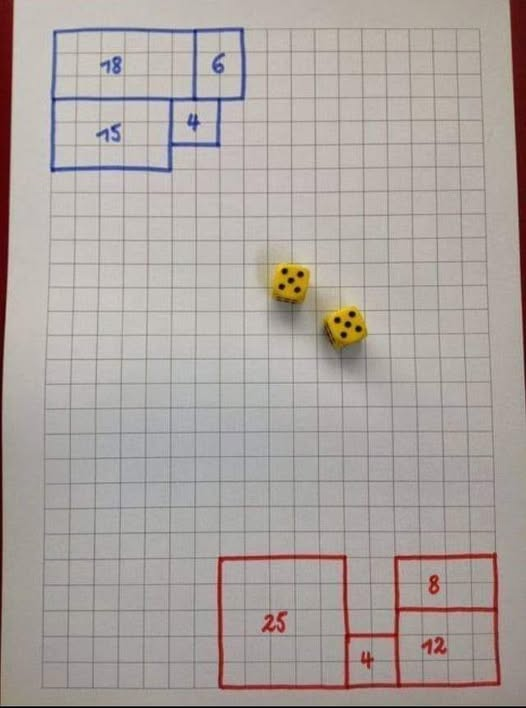
\includegraphics[width=0.45\textwidth]{images/jeu_carre_aire.jpg}
    \end{center}
\end{multicols}

\vspace{-0.7cm}\subsection{Juniper Green}

\input{Juniper_green/test_autojeu_refill} % Inclusion de l'énoncé

\newpage 

\subsection{Multiplicato}

\input{Juniper_green/autojeu_multiplicato} % Inclusion de la solution

